\subsection{《说中国》}

作者:许倬云

\subsubsection{标注}

1. “中国”这个观念维系力量有三,一是经济网络,二是政治精英,三是书写文字。

2. 特别强调不同的生产方式和生活方式,如何使不同的族群与文化逐渐杂糅、融合与交错。

3. 如果说《万古江河》重点在讨论中国的“历史”和“文化”,《我者与他者》重点在讨论历史与文化中的中外关系,那么这本《华夏论述》重点就是在讨论历史与文化中“中国”之变动。

4. 欧洲人从新大陆取得巨量白银,其中至少有三分之一甚至一半流入中国。

5. 我(作者)将“中国”看作是一个复杂体系的共同体。

6. 我习惯上使用系统论的方法分析历史现象,尤其所谓“大历史”的研究方法,不能从单独的事件着眼,必须从各种现象的交互作用来观察整体的变化。

7. 蒙古和满清,两次征服中国全部地区,在中国历史上留下深刻的烙印:最沉重之影响,应当是完全倚仗暴力压制的统治形态。于是,中国传统的“天命”观念,及“天命”应建立在“民视”、“民听”基础之上的相对性,经过上述全盘暴力镇压的残酷现实,竟从此再不能支持百姓对绝对皇权的抵抗。

8. 定期察举,等于将全国人不断地周转,不使任何地方独占权力,也使全国的信息因为人才流转而流转,全国的政策不至于有地方性的偏差。

9. 华”是华美,“夏”是伟大——华美而伟大的文化,就是“华夏”,

10. 台湾原居民的语言是南岛语系的源头。由此可以推知,南岛语系的祖源其实就是包括所谓“百越”在内的东南人群。

13. 离现在一万年前左右,黄牛第一次被驯养为家畜。

\subsubsection{新石器时代华夏文明的演进}
这一部分内容比较有价值,梳理了夏之前华夏文明的区域化出现、融合和消亡。
\begin{figure}[htpb]
\centering
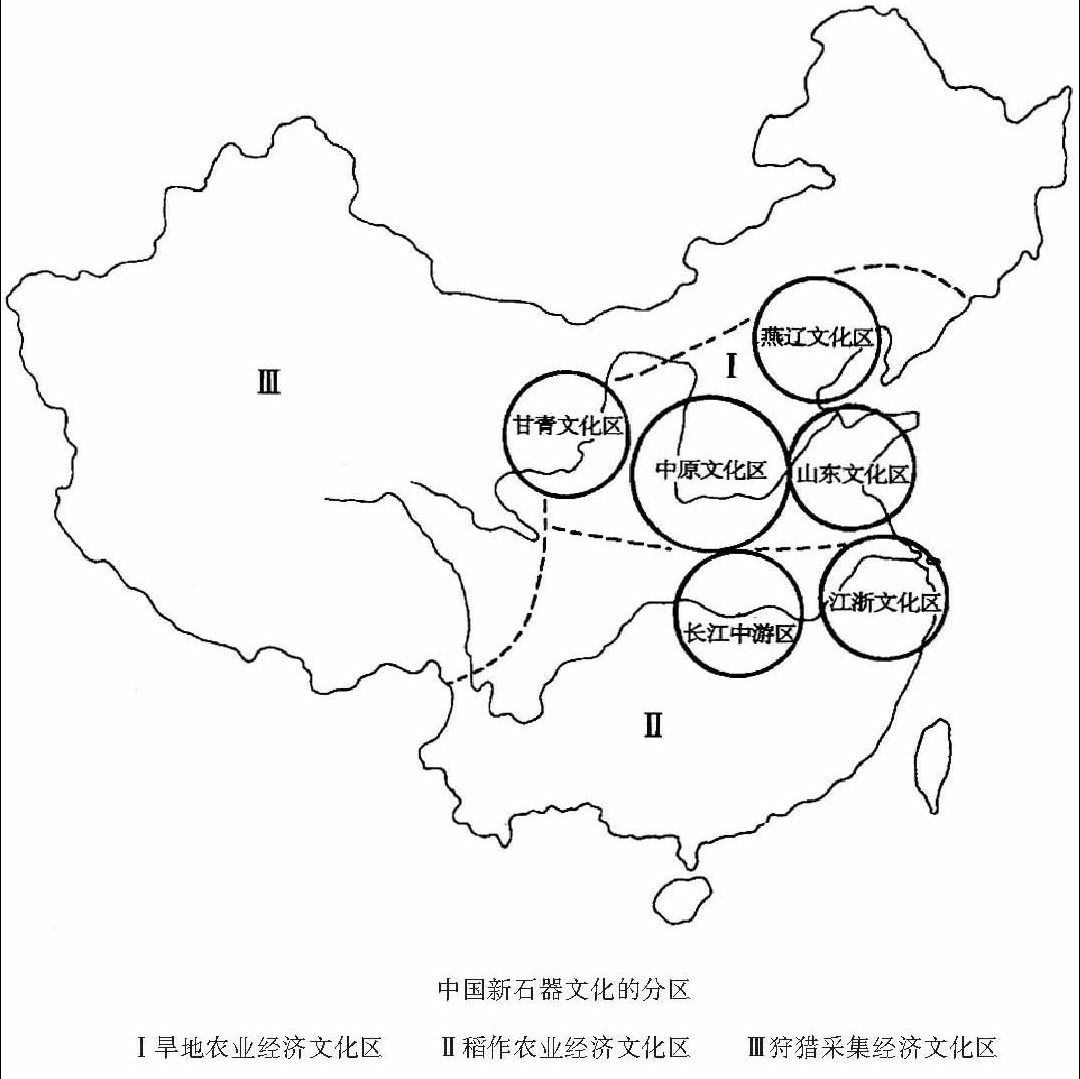
\includegraphics[width=0.8\linewidth]{images/china-ancient.png}
\caption{中国古文明分布图。}
\end{figure}

\begin{enumerate*}
	\item 湖南江西地区,九千年前耕作水稻,为东方第一次,村落产生在离水比较近的高地上或平地的灌溉系统上。水稻耕作进入北方(如汉水流域)
	\item 东北地区,一万年前黄牛被驯化,村落产生在向阳的山坡或山谷上。
	\item 太行山东部到渤海间的山坡地上,七八千年前,人类发展了粟(小米),村落产生在离水既不太近也不太远的二道塬上。
	\item 此时人类族群的分野,并非以血缘为基本要素,而是以生活方式当作认同的文化基因。
	\item 畜牲文化构火而居,因此称为“狄”;携长弓的渔猎部族,称为“夷”;种植小米的人刀耕火种,称为“烈山氏”“神农”“后稷之后”,“周”是田野的象征。
	\item 六七千年前,中国各地的村落已经有较大规模,并产生了贫富分化和阶级。东北辽河的红山文化有大型酋长墓葬和祭坛,具有母性形象的神明、雕刻精神的玉器;浙江的良渚文化也出现了土山的祭坛、玉琮和宫殿遗址;山东大汶口文化中,村落庞大,有黑陶及之上的文字;汉口流域和长江中游之间存在种植水稻的文化,如石家河文化的城市遗址。
	\item 四五千年前出现了长期干旱,北方草原文明南移,陕西神木发现石峁文化。
	\item 历史传说可能与当时的集体记忆有关,例如五帝之间的斗争,其中炎帝是农业民族(神农),颛顼是制定农耕历法的民族,太昊、少昊是以鸟类为图腾的太阳神崇拜者,以上四者均在渤海冲积平原上,黄帝是胜利者,“以师兵为营卫”,是一个战斗族群。
\end{enumerate*}

\begin{figure}[htpb]
\centering
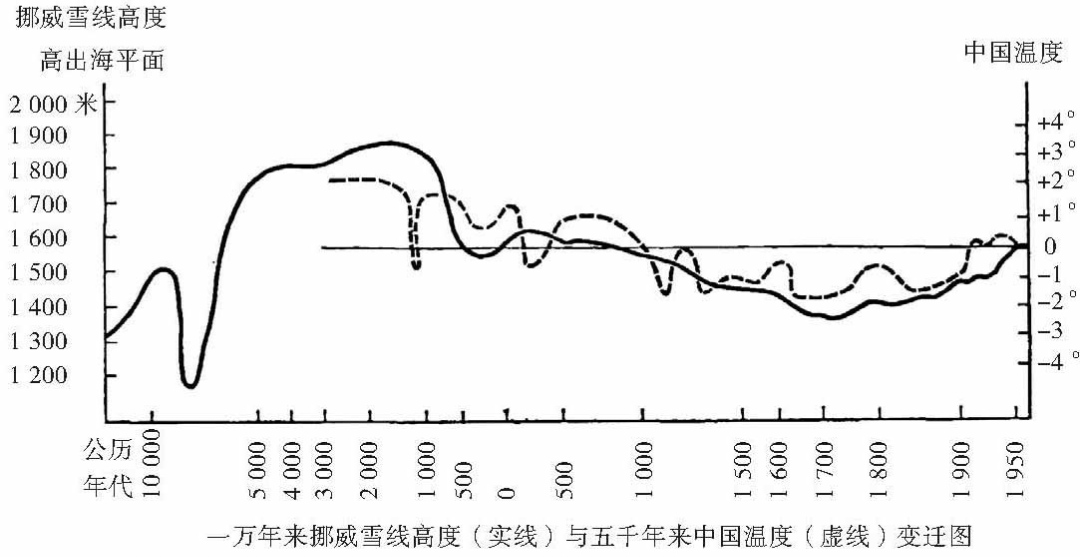
\includegraphics[width=0.8\linewidth]{images/china-tem.png}
\caption{中国古代气温变化。}
\end{figure}

四千年前,夏朝产生,其他上述文化均退化迁徙(例如大汶口文化南迁,与良渚文化交融,带入黑陶烧制技术,而台湾史前玉器文化与良渚文化相近),人口出现交融,例如源自台湾的“南岛语系”可能与百越文化有渊源。

\subsubsection{夏商周}
渤海外围的族群南迁时,遇见黄河中游的夏文化,并交融。此时二里头文化已经经过河西走廓与中亚、西亚文明有交流,引入麦类作物和青铜器。

商人来自渤海地区,崇拜高天(玄鸟生商),商代统治区域扩大,超出“中原”范围。

周人本居陕北和晋西,原本务农,但在气候变冷时也牧养。

\subsubsection{书评}

书名为《说中国》,实际上论述的是中国这一文化共同体的发展变化。本书是许倬云结合人类学、考古成果和中国基本历史(包括政治制度演变、经济重心转移等)对中国历史的梳理,内容不多,篇幅不长,却值得一读。

中国不仅仅是一个地理概念,更重要的是一个文化概念。在中国这片土地上,自新石器时代起,地理范围和文化内涵就在不断变化,两者是一个相互牵制、相互影响的过程。史前时代华夏大地的不同部落,经过长期的战争、迁徙和融合,不断扩大“华夏”这一范围的边界,并最终形成现在的广大农业区。这一农业区的边界,是牧业区(北部)或地理阻隔。于是在这样一个土地上,华夏文明生根发芽,不曾中断。并且,华夏文明与周边的文明进行碰撞、交融,但没有失去自己的主体性和延续性,这在人类文明史上是独一无二的。

在这种流变中,文化(统一的文字、历史记忆、儒家学说等)与经济相互牵制将广大地域和不同文化习俗捏合在一起。一旦有了外族入侵(如三国后期),联结在一起的各个区域之间由于有经济上的依赖性,因此无法分割开来,使得割据一方成为不可能。汉朝奠定了华夏文明的疆土和文化认同,唐朝有了进一步发展,这在许倬云看来都是十分耀眼的,是中华的“正统”。宋代并不占有全部的“天下”,而元明清三代的奴化压迫较为严重,在许倬云看来失去了华夏的气度。这里许倬云明显受到了日本人近代的影响,并且有一定的台独倾向,将元明清(特别是明朝的改土归流)与殖民等同,其史观令人惊讶。沿着他的说法,日本殖民中国的正当性就有了,台湾独立的合法性也有了,这是十分错误了。在我看来,元明清虽然有其弊端,但整体上都是华夏文化的传承,虽然后来越来越封闭,但这没有背离华夏文明的传统,因此对其贡献应当予以承认。

因此,这本书前半部值得一看,后半部便失了水准,读者应当对其内容选择性和批判性吸收。

评分:3/5。